\documentclass[12pt]{article}
\usepackage[utf8]{inputenc}
\usepackage{float}
\usepackage{amsmath}
\usepackage{graphicx}

\usepackage[hmargin=3cm,vmargin=6.0cm]{geometry}
%\topmargin=0cm
\topmargin=-2cm
\addtolength{\textheight}{6.5cm}
\addtolength{\textwidth}{2.0cm}
%\setlength{\leftmargin}{-5cm}
\setlength{\oddsidemargin}{0.0cm}
\setlength{\evensidemargin}{0.0cm}

%misc libraries goes here


\begin{document}

\section*{Student Information } 
%Write your full name and id number between the colon and newline
%Put one empty space character after colon and before newline
Full Name :  Murat TOPAK\\
Id Number :  2036218\\

% Write your answers below the section tags
\section*{Objective}
%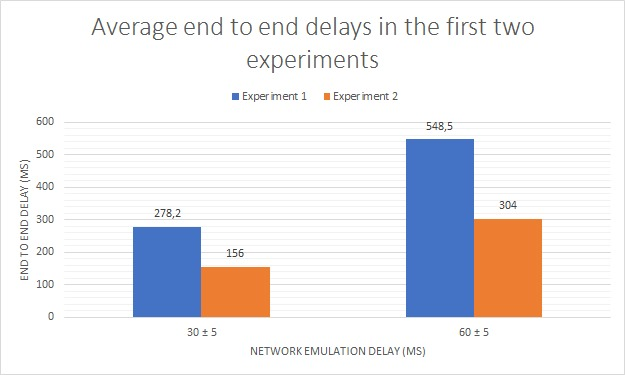
\includegraphics[scale=0.8]{graph.jpg}

The homework wants us to write our own protocol, and compare it to one of transport layer protocols of the Internet. More specifically, we are allowed to use only UDP sockets, asked to develop an RDT at the transport layer, and measure its performance against SCTP.
The code to experiments is all written in Python. An open source library, PySCTP, has been used to meet the requirements of the homework. On the other hand, Selective-Repeat(SR), rather than Go-Back-N(GBN) is our solution regarding the RDT. The reason to go with SR is that GBN would be disastrous since it re-sends all of the packets belonging to a window in case one of them is lost or corrupted. Since we have a high rate of corruption and loss in some of the experiments, this would definetely slow down the process. For the multihoming, we use a multi-threaded approach to utilize the two links at the same time.



\section*{Figure 1}

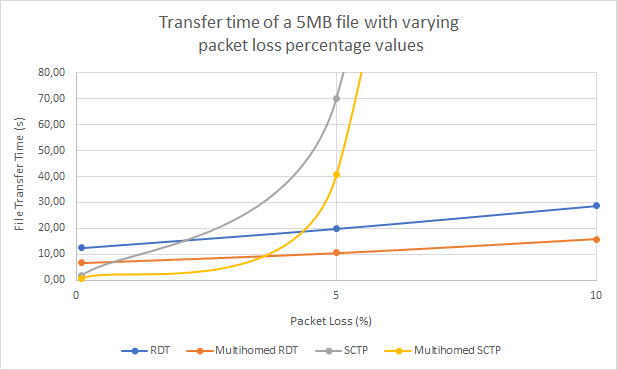
\includegraphics[scale=0.8]{graph1.png}
\\\\
In the figure, the transfer time of a 5MB file is given with respect to different packet loss percentage values. First thing we have noticed here is that SCTP reacts exponentially to packet loss while our RDT follows a linear fashion. This makes sense because PySCTP library uses TCP style sockets to implement SCTP. We know TCP has congestion control mechanisms. Each packet loss leads to a decline in the throughput of the link because of these underlying mechanisms like TCP-Reno or TCP-Tahoe. Moreover, each timeout contributes to an increase in the timeout value of TCP. This makes it almost impossible to send the file with a 10\% packet loss. At first, this seemed abnormal but after a research, we understood this was indeed supposed to be the case.\\
\\Mathis formula relates the TCP throughput with $\dfrac{MSS}{RTT\sqrt{p}}$, where the variables represent maximum segment size, round-trip-time, and packet loss probability. In our case, we have $MSS = 256$ bytes, $RTT = 13$ ms, and $p = 10$. It can be verified that the formula yields $50$kbps for the actual throughput of the link.
\\\\In contrast to SCTP's exponential behaviour, our RDT does not suffer from the above issues. It is because there is neither congestion control nor dynamic timeout calculation in our RDT. Our window size, and timeout value stays the same during all of the transmission.  This makes our protocol work in a linear time with respect to packet loss. This comparison between SCTP and RDT showed us the real life protocols are great but not in every case. In these cases, people should write their own protocol considering the environment.\\\\
Besides from SCTP vs RDT, we see our multihoming works as expected. The time needed for transmission gets almost halved in the multihomed approach, regardless it is SCTP or RDT.


\section*{Figure 2}

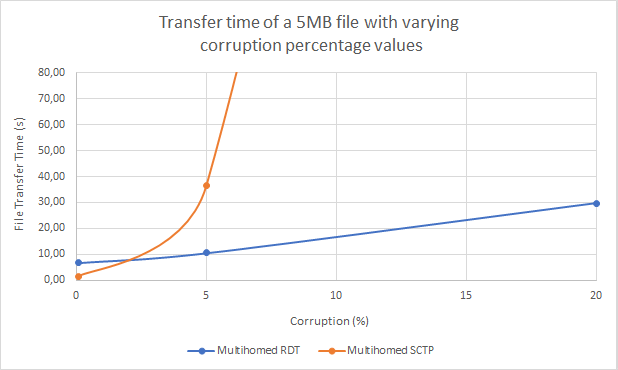
\includegraphics[scale=0.8]{graph2.png}
\\\\
This figure illustrates the relation between the file transfer time and corruption percentages. This is actually not much different than the packet loss case. SCTP uses TCP sockets as explained above. TCP offers no exclusive mechanism to corruption than it offers to packet loss. On the other hand, our protocol is so naive it does not take any special action when the packet is lost or corrupted. Therefore, the curves look similar to multihomed protocols of the first figure.\\\\ One thing to note here is that, the transfer time is almost 30 seconds when the corruption percentage is 20\%. Recall that it was around 15 seconds when the packet loss percentage was 10\%. This is just another way of showing the corruption follows the linear curve of the packet loss. Hence, whether it is a packet loss or corruption, SCTP reacts exponentially, and RDT reacts linearly to the changes in the percentages.


\section*{Figure 3}

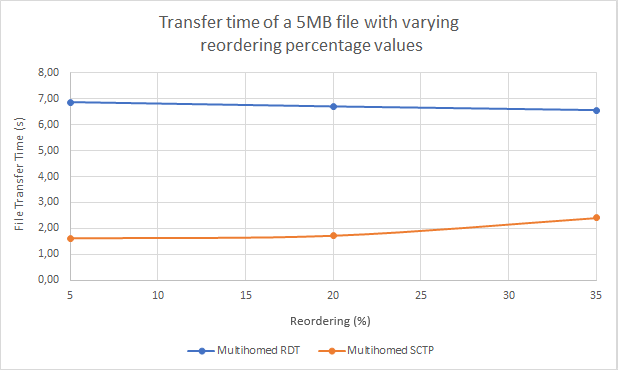
\includegraphics[scale=0.8]{graph3.png}
\\\\
This figure relates the file transfer time to reordering percentage. It tries to illustrate how the protocols react when the packets arrive out of order. We see the reordering does not really affect the performance of the two protocols. This is because TCP buffers the out-of-order data, and so does our protocol despite its simpleness. Thus, no serious bottlenecks are present, whether it is SCTP, or RDT.\\\\
Our protocol may seem slow here, but actually this is its best performance. When the packet loss and corruption parameters are set back to normal as in this figure, SCTP beats us in time since it is a well-designed protocol for real life.

\section*{Others}
To calculate the sample size $n$ at 95\% confidence, the formula is $MoE = \dfrac{0.98}{\sqrt{n}}$. When solved for $n$ with $MoE=0.025$, it gives 1536. Since the standard error is so small at this size, there are not any confidence intervals drawn as they would uglify the figures, and not even get noticed.\\\\
More technical detail like routing, packet structure, and implementation can be found in the README and in the source codes.


\end{document}

​
